\section{Data acquisition}

The second phase of the pipeline is data acquisition. After we have set up the camera according to the session parameters we can start recording. We set a timer for $30s$ and record the RGB and Depth streams from the camera. We also record the camera intrinsics, which we will use to recreate the point cloud at a later stage. We record the data in a folder structure that is defined by the session parameters.

\subsection{Data format}

An important part of data acquisition is the description of the way the data is stored in the file system. This is essential for any future use of the data and therefore we need to make sure that the data is stored in a way that is easy to understand and easy to use. We store in general two to five files per session depending on the camera configuration. 

\subsubsection{Session Metadata}

Every session contains a "\texttt{SESSION\_NAME.json}" file that contains the session parameters and camera metadata. The session name is automatically generated based on the starting time of the session, this way we can make sure that the session name is unique every time and we can also have an idea of which recording is the most recent without looking at the contents of the file.

\paragraph{Camera metadata}

The camera metadata contains the camera intrinsics, which we will use to recreate the point cloud at a later stage. The camera intrinsics are the field of view of the depth camera in the horizontal and vertical direction, and the principal point in the horizontal and vertical direction. The field of view is the angle between the optical axis and the image plane. The principal point is the point in the image where the optical axis of the camera intersects the image plane. The principal point and the field of view are explained in Figure \ref{fig:pinhole_camera_model}.

\begin{figure}[ht]
  \centering
  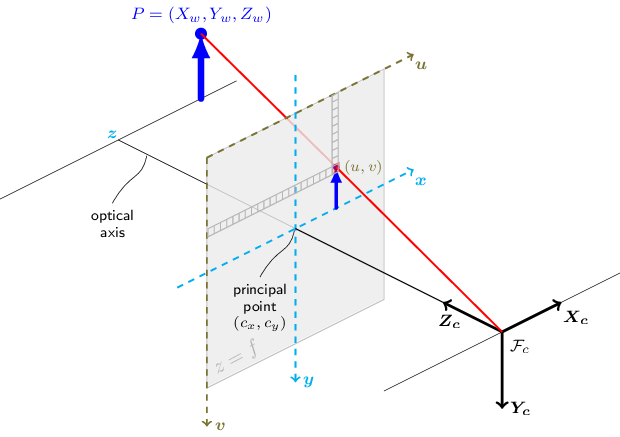
\includegraphics[width=.9\textwidth]{figures/CameraCalibration/pinhole_camera_model.png}
  \caption[Pinhole camera model]{The pinhole camera model showing the principal point. The principal point is the point where the optical axis intersects the image plane. The field of view is the angle between the optical axis and the image plane.}
  \label{fig:pinhole_camera_model}
\end{figure}

\paragraph{Camera orientation}

Additionally, to the camera intrinsics we store the relative rotation and translation between the cameras if multiple cameras are used. The rotation and translation are stored as Euler angles\footnote{Technically we are storing the rotation with the Tait–Bryan notation, i.e. x-y-z or yaw-pitch-roll, rather than the classic Euler notation. However, the name Euler angle is more commonly used and understood.} and a vector respectively \cite{euler1776formulae}. The rotation is the rotation of the camera relative to the second camera in the system. The translation is the translation of the camera concerning the second camera in the system.

\paragraph{Session parameters}

The session parameters are the same as the ones defined in the section "Stream pre-processing". The user enters the session parameters before starting the recording. Most of the parameters are boolean values that indicate whether the user is sitting, wearing dark clothing, etc. The height and angle parameters are the height of the camera to the floor and the angle of the camera relative to the orientation of the user as explained in the previous section.

An example of the Session metadata can be seen in Listing \ref{lst:session_metadata}.

\begin{lstlisting}[language=json,
                   firstnumber=1,
                   caption={[Example of session metadata]{Example of the Session metadata with a single Realsense Camera which was recorded for 40 seconds at around 30 frames per second resulting in 1200 frames. Some values have been changed to increase readability.}},
                   label={lst:session_metadata}]
{
  "Cameras" : 
  [
    {
      "Cx" : 314.26,
      "Cy" : 239.46,
      "FileName" : "Session_2023-01-30T09.21.34_Realsense_Camera_0.bag",
      "Fx" : 459.77,
      "Fy" : 459.83,
      "MeterPerUnit" : 0.00025,
      "Name" : "Realsense Camera 0",
      "Type" : "Realsense"
    }
  ],
  "DurationInSec": 40.0,
  "Name": "Session 2023-01-30T09:21:34",
  "RecordedFrames": 1200,
  "Rotation": {
      "Roll": 0.0,
      "Pitch": 0.0,
      "Yaw": 0.0
  },
  "Translation": {
      "X": 0.0,
      "Y": 0.0,
      "Z": 0.0
  },
  "Session Parameters": {
    "Sitting": true,
    "Background close": true,
    "Cramped": false,
    "Dark Clothing": true,
    "Holding Weight": false,
    "Ankle Weight": false,
    "Height": 1.8,
    "Angle": 20.0
  }
}
\end{lstlisting}

\subsubsection{Session Metadata}